%!TEX root = main.tex
\setcounter{chapter}{3}
\setcounter{section}{7}
\setcounter{theorem}{0}
\setcounter{equation}{0}

\lectureheader{161}{Calculus I}{Implicit differentiation}{\textit{Thomas' Calculus} \thesection}

\begin{example}
Compute the slope of the tangent line to the circle $x^2+y^2=25$ at the point $(3,4)$.
What about at the point $(4,-3)$?
\end{example}
\begin{flushright}
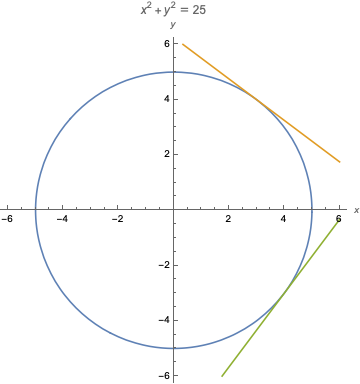
\includegraphics[width=3in]{img/circle}
\end{flushright}

\newpage

\begin{remark}\,
\begin{enumerate}
\item The graph of an equation in the variables $x$ and $y$ typically is a curve in the $xy$-plane.
\item A typical curve in the $xy$-plane does not satisfy the vertical line test, and so we cannot solve for $y$ \textit{uniquely} as a function of $x$.
\item Nevertheless, we can still compute slopes of tangent lines to the curve using a technique called \textbf{implicit differentiation}.
\item To implicitly differentiate $y$ with respect to $x$\dots
\begin{enumerate}
\item Differentiate both sides of the equation with respect to $x$, viewing $y$ as a differentiable function of $x$ and applying the chain rule appropriately.
\item Solve for $\DS\frac{\dee y}{\dee x}$.
\end{enumerate}
\end{enumerate}
\end{remark}

\begin{example}
Use implicit differentiation to compute a formula for the slope of the tangent line to the circle $x^2+y^2=25$ at each point $(x_0,y_0)$ on the circle.
\end{example}

\newpage

\begin{example}
Show that the point $(2,4)$ lies on the curve $x^3+y^3-9xy=0$.
Then find equations for the tangent and normal line to the curve at that point.
\end{example}
\begin{flushright}
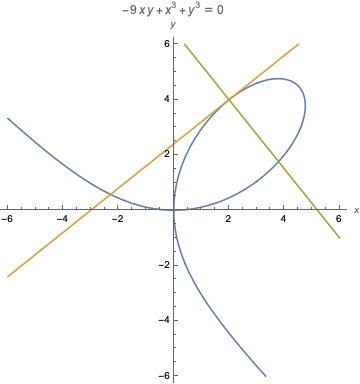
\includegraphics[width=3in]{img/tangent_and_normal_example}
\end{flushright}

\newpage

\begin{example}
Compute $\dee y/\dee x$ if $y^2=x^2-\sin xy$.
\end{example}

\newpage

\begin{example}
Compute $\dee^2y/\dee x^2$ if  $2x^3-3y^2=8$.
\end{example}

\newpage


\begin{example}
Show that at every point except for $(x,y)=(0,0), (\pm 1, 0)$, the tangent line to the curve $y^2=x^3-x$ meets the curve in exactly one other point.
\end{example}
